% Part: model-theory
% Chapter: interpolation
% Section: separation

\documentclass[../../../include/open-logic-section]{subfiles}

\begin{document}

\olfileid[fr]{mod}{int}{sep}
\olsection{Séparation des \printtoken{p}{sentence}}

Il nous faut quelques résultats préliminaires
avant de démontrer le théorème d'interpolation.
Un interpolant de~$!A$ et~$!B$ est
!!a{sentence}~$!C$ tel que
$!A\Entails !C$ et $!C\Entails !B$.
Par contraposition, la seconde condition
équivaut à $\lnot !B\Entails\lnot !C$.
Un tel !!{sentence}~$!C$ \emph{sépare}
donc~$!A$ de~$\lnot !B$.
Chercher un interpolant revient ainsi
à chercher un !!{sentence} qui sépare
ces deux énoncés. Comme souvent, il sera
utile de généraliser cette notion à la
séparation de deux \emph{ensembles}
d'!!{sentence}s.

\begin{defn}
Un !!{sentence}~$!C$ \emph{sépare}
les ensembles d'!!{sentence}s
$\Gamma$ et~$\Delta$ si et seulement si
$\Gamma\Entails !C$ et
$\Delta\Entails\lnot !C$.
S'il n'existe pas de tel !!{sentence},
$\Gamma$ et~$\Delta$ sont
\emph{inséparables}.
\end{defn}

La figure suivante représente les
inclusions entre les classes de modèles
de~$\Gamma$, de~$\Delta$ et de~$!C$ :
\begin{figure}[h]
  \centering
  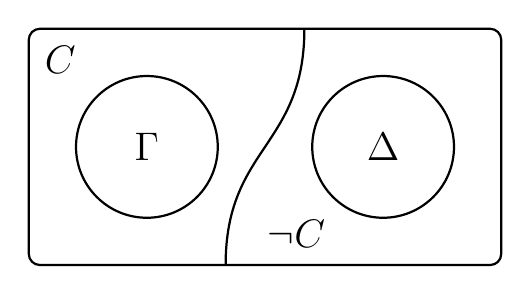
\begin{tikzpicture}[node distance=2cm, auto, thick]
    \draw [rounded corners] (0,0) -- (6,0) -- (6,3) -- (0,3) -- cycle;
    \draw (1.5,1.5) circle (0.9cm);
    \draw (4.5,1.5) circle (0.9cm);
    \path node at (1.5,1.5) {\Large $\Gamma$};
    \path node at (4.5,1.5) {\Large $\Delta$};
    \path node at (0.4,2.6) {\Large $\formula{C}$};
    \path node at (3.4,0.4) {\Large $\lnot\formula{C}$};
    \draw (2.5,0) .. controls (2.5,1.5) and (3.5,1.5) .. (3.5,3);
  \end{tikzpicture}
  \caption{$!C$ sépare $\Gamma$ et $\Delta$}
  \ollabel{fig:sep}
\end{figure}

\begin{lem}
\ollabel{lem:sep1}
Soit $\Lang{L}_0$ le langage qui contient
toutes les !!{constant}s,
les !!{function}s et les !!{predicate}s
autres que~$\doteq$ figurant à la fois
dans~$\Gamma$ et dans~$\Delta$.
Soit $\Lang{L}'_0$ le langage obtenu
en lui adjoignant une infinité de
nouvelles !!{constant}s
$\Obj c_n$, pour $n\geq0$, ne figurant ni dans~$\Gamma$ ni dans~$\Delta$.
Si $\Gamma$ et~$\Delta$ sont
inséparables dans~$\Lang{L}_0$,
ils le restent dans~$\Lang{L}'_0$.
\end{lem}

\begin{proof}
Raisonnons par l'absurde. Supposons qu'un
!!{sentence}~$!D$ de~$\Lang{L}'_0$
sépare $\Gamma$ et~$\Delta$.
Il ne contient qu'un nombre fini de
nouvelles constantes. S'il n'en contient
aucune, il sépare déjà les deux ensembles
dans~$\Lang{L}_0$, ce qui est impossible.
Traitons le cas où seule~$c$ y figure,
et, après renommage des variables liées pour éviter toute capture de~$x$, écrivons
$!D=\Subst{!C}{c}{x}$,
où $!C$ est une !!{formula} de~$\Lang{L}_0$
dont $x$ est la seule !!{variable} libre
éventuelle.
Par compacité, il existe des sous-ensembles
finis $\Gamma_0\subseteq\Gamma$ et
$\Delta_0\subseteq\Delta$ tels que
$\Gamma_0\Entails\Subst{!C}{c}{x}$
et
$\Delta_0\Entails\lnot\Subst{!C}{c}{x}$.
Notons $!G$ et~$!H$ les conjonctions
respectives de ces ensembles finis
(une conjonction vide étant une tautologie).
Ainsi,
\begin{align*}
  !G &\Entails\Subst{!C}{c}{x},
  &
  !H &\Entails\lnot\Subst{!C}{c}{x}.
\end{align*}
Puisque $c$ est nouvelle et ne figure
ni dans~$!G$ ni dans~$!H$,
$!G\Entails\lforall[x][!C]$ et
$!H\Entails\lforall[x][\lnot !C]$.
En particulier,
$!H\Entails\lnot\lforall[x][!C]$.
Par monotonie,
\begin{align*}
  \Gamma &\Entails\lforall[x][!C],
  &
  \Delta &\Entails\lnot\lforall[x][!C].
\end{align*}
Le !!{sentence}~$\lforall[x][!C]$
séparerait donc $\Gamma$ et~$\Delta$
dans~$\Lang{L}_0$, contradiction.\footnote{Corrections éditoriales : la lettre $\delta$ non définie dans la preuve source renvoie à la conjonction $!H$. Nous distinguons la formule $!C$ de l'énoncé fermé obtenu par quantification, puis explicitons l'élimination successive des constantes nouvelles.}
Si~$!D$ contient plusieurs nouvelles
constantes, on en choisit une et
on applique le même raisonnement
dans le langage qui contient encore
toutes les autres. Chaque étape
diminue leur nombre; on finit donc
par obtenir un séparateur dans
$\Lang{L}_0$, contradiction.
\end{proof}

\begin{lem}
\ollabel{lem:sep2}
Supposons que
$\Gamma\cup\{\lexists[x][!S]\}$
et~$\Delta$ soient inséparables.
Soit~$c$ une nouvelle !!{constant}
qui ne figure ni dans~$\Gamma$,
ni dans~$\Delta$, ni dans~$!S$.
Alors
$\Gamma\cup
\{\lexists[x][!S],\Subst{!S}{c}{x}\}$
et~$\Delta$ sont également inséparables.
\end{lem}

\begin{proof}
Supposons au contraire qu'un
!!{sentence}~$!C$ sépare
$\Gamma\cup
\{\lexists[x][!S],\Subst{!S}{c}{x}\}$
de~$\Delta$, tandis que
$\Gamma\cup\{\lexists[x][!S]\}$
et~$\Delta$ restent inséparables.
Distinguons deux cas :
\begin{enumerate}
\item Si $c$ ne figure pas dans~$!C$,
  l'ensemble
  $\Gamma\cup\{\lexists[x][!S],\lnot !C\}$
  est satisfaisable; sinon~$!C$
  séparerait déjà
  $\Gamma\cup\{\lexists[x][!S]\}$
  de~$\Delta$. Dans un modèle de cet
  ensemble, on interprète~$c$ par un
  témoin de~$\lexists[x][!S]$.
  Le modèle obtenu satisfait aussi
  $\Subst{!S}{c}{x}$ et~$\lnot !C$,
  contrairement au choix de~$!C$.
\item Si $c$ figure dans~$!C$,
  écrivons $!C=\Subst{!D}{c}{x}$,
  après renommage des variables liées pour éviter toute capture de~$x$, avec $!D$ ne contenant pas~$c$ et dont la seule variable éventuellement libre est~$x$.
  L'hypothèse donne
  \[
  \Gamma\cup
  \{\lexists[x][!S],\Subst{!S}{c}{x}\}
  \Entails\Subst{!D}{c}{x}.
  \]
  Comme~$c$ est nouvelle,
  le théorème de déduction et la
  généralisation donnent
  $\Gamma\cup\{\lexists[x][!S]\}
  \Entails\lforall[x][(!S\lif !D)]$,
  donc
  $\Gamma\cup\{\lexists[x][!S]\}
  \Entails\lexists[x][!D]$.
  D'autre part,
  $\Delta\Entails
  \lnot\Subst{!D}{c}{x}$,
  d'où, par la même fraîcheur de~$c$,
  $\Delta\Entails\lnot\lexists[x][!D]$.
  Le !!{sentence}~$\lexists[x][!D]$
  séparerait donc les deux ensembles
  supposés inséparables : contradiction.\footnote{Corrections éditoriales : nous distinguons ici le séparateur $!C$ de la formule $!D$ avant substitution et rétablissons les crochets du second argument de la macro existentielle dans l'hypothèse de la preuve source.}
\end{enumerate}
\end{proof}

\end{document}
